\section{Ergebnisse}
%xy anpassen!!!
Die in Abschnitt 3.2 beschriebene Netzstruktur wird mit dem in Abschnitt 3.3 vorgestelltem Datensatz und Parametern trainiert und validiert. Die optimalen Trainingsparameter wurden dabei aus mehren Experimenten empirisch ermittelt. Dabei dient die in Abschnitt 3.1 erarbeitete \textit{Loss}-Metrik zur jeweiligen Quantisierung des Trainingserfolges. \\Abbildung \ref{lossbild} zeigt den Verlauf des \textit{Loss} über die Trainingsiterationen im 3D-Fall. Die Variable \textit{loss} steht für den \textit{Loss}  der Trainingsdaten und \textit{val\_loss} für den \textit{Loss} der Testdaten. Dabei fällt dieser zunächst relativ schnell und nähert sich dann XY an. Dies deutet auf ein erfolgreiches Training ohne \textit{Overfitting} hin. 
%\begin{figure}[!htb] %loss und val_loss graph
%  \centering
%  \includegraphics[width=6.8cm]{}
%  \caption{Loss und Val_loss über Trainingsepochen}
%  \label{lossbild}
%\end{figure} 
In Abbildung werden beispielhaft einige prädizierte Bounding-Boxen der Testdaten dargestellt (blau). Zum Vergleich sind zusätzlich die manuell vorgelabelten Bounding-Boxen eingezeichnet (rot). Oben im Bild steht der jeweils errechnete \textit{Loss}. Hier ist zu erkennen, dass das mittlere Bild mit dem höchsten \textit{Loss} auch die sichtbar größte Abweichung der prädizierten Bounding-Box mit der vorgelabelten aufweist. Der \textit{Loss} im linken und rechten Bild ist relativ ähnlich und spiegelt so auch die erkennbar ähnliche Abweichung der beiden Bounding-Boxen wieder.\\ \label{pred_boxes}
\begin{figure}[!htb]
  \centering
  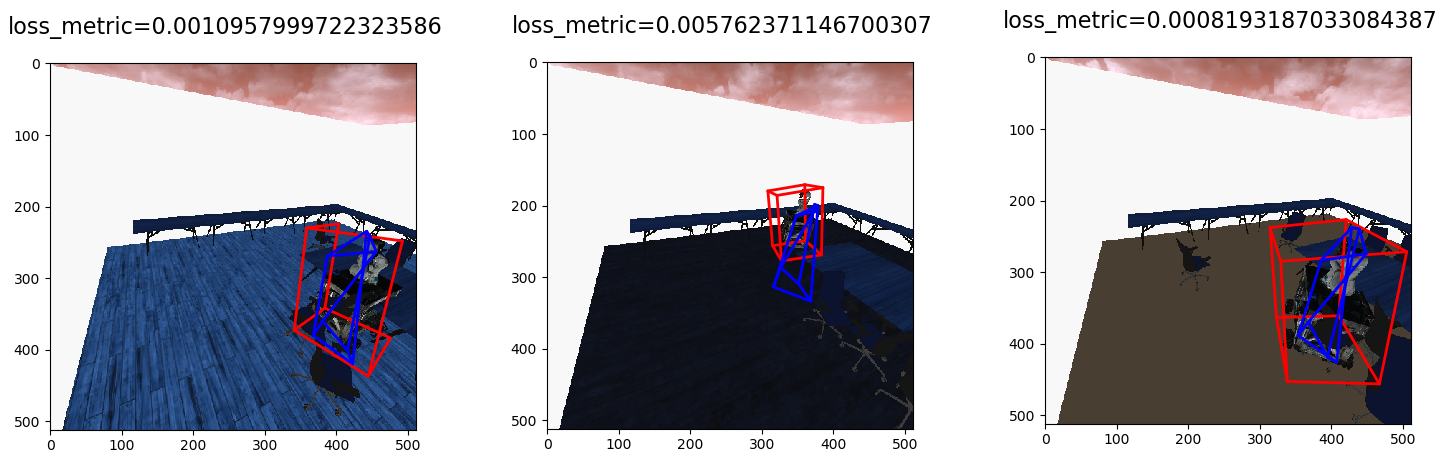
\includegraphics[width=13.8cm]{Abb/pred_bb.png}
  \caption{Trainierte und prädizierte Bounding-Boxen}
  \label{pred_boxes}
\end{figure} 
